\documentclass{standalone}
\usepackage{ tikz }
\usepackage{ xparse }
\usepackage{../../../macros}

\begin{document}
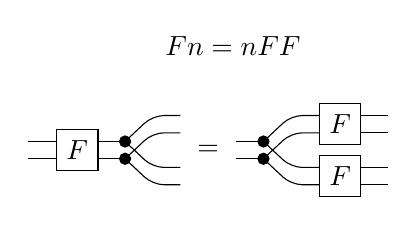
\begin{tikzpicture}[yscale=-1,x=1em,y=1.25em]

    \draw (0.5,-0.25) -- (1.5,-0.25);
    \draw (0.5,0.25) -- (1.5,0.25);
    \node[draw, minimum height = 1.5em, minimum width = 1.5em, anchor = west] at (1.5,0){$F$};
    \draw (3,-0.25) -- (4,-0.25);
    \draw (3,0.25) -- (4,0.25);
    \filldraw (4,-0.25) circle (2pt);
    \filldraw (4,0.25) circle (2pt);
    \draw [rounded corners] (4,-0.25) -- (5,-1) -- (6,-1);
    \draw [rounded corners] (4,-0.25) -- (5,0.5) -- (6,0.5);

    \draw [rounded corners] (4,0.25) -- (5,-0.5) -- (6,-0.5);
    \draw [rounded corners] (4,0.25) -- (5,1) -- (6,1);

    \node at (7,0) {$=$};
    \node at (7.9,-3) {$F \seq \ccopy{n} = \ccopy{n} \seq F \tensor F$};

    \draw (8,-0.25) -- (9,-0.25);
    \draw (8,0.25) -- (9,0.25);
    \filldraw (9,-0.25) circle (2pt);
    \filldraw (9,0.25) circle (2pt);
    \draw [rounded corners] (9,-0.25) -- (10,-1) -- (11,-1);
    \draw [rounded corners] (9,-0.25) -- (10,0.5) -- (11,0.5);

    \draw [rounded corners] (9,0.25) -- (10,-0.5) -- (11,-0.5);
    \draw [rounded corners] (9,0.25) -- (10,1) -- (11,1);

    \node[draw, minimum height = 1.5em, minimum width = 1.5em, anchor = west] at (11,-0.75){$F$};
    \node[draw, minimum height = 1.5em, minimum width = 1.5em, anchor = west] at (11,0.75){$F$};

    \draw (12.5,-1) -- (13.5,-1);
    \draw (12.5,-0.5) -- (13.5,-0.5);
    \draw (12.5,0.5) -- (13.5,0.5);
    \draw (12.5,1) -- (13.5,1);

\end{tikzpicture}
\end{document}